
\begin{figure*}
\begin{center}
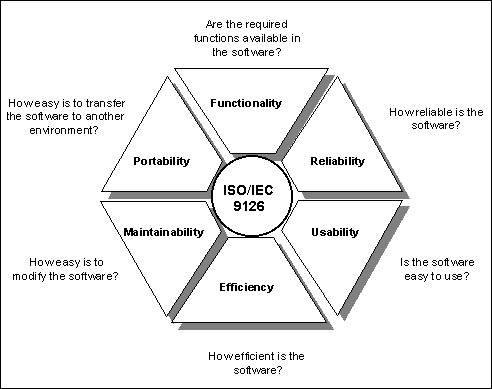
\includegraphics[scale=0.8]{9126ref.png}
\caption{Shows the diffrence between the Test-Last and Test-First workflow}
\end{center}
\end{figure*}

Software is defined from software quality assurance perspective as “combination of computer program (the “code”), procedures, documentation, and data necessary for operating the software the system”~\cite{Galin}. The Software Quality on the other hand defines according to Pressman is “ the degree of conformance to specific functional requirements, specific software quility and Good Software Engineering Practices (GSEP) “~\cite{Pressman}.

This report uses code quality as a term for both “software functional quality” and “Software structural quality” or “Non-functional quality” as Lawrence and Julio~\cite{Chung} describe it where the first one refers more to code per se and the later more to the behavior of the code such as software affection or usability. 

Code quality could be defined and categorized in numerous ways and it has been standardized differently in the past. There is an international standard for product quality ISO-9126 and ISO-25000~\cite{ISO9126}  which defines a basic quality model. This report uses these standard to define Code quality but also the global standard made by “Consortium for IT Software Quality” about business value and costumer satisfaction \url{(http://www.it-cisq.org/cisqwiki/images/8/87/CISQ_2009_Executive_Forums_Report.pdf)} which is based above mentioned standards. 

ISO-9126 is an international standard for product quality and defines six major desirable characteristics which ought to measured in order to guarantee good code quality. Each characteristic is divided into sub-characteristic and further split into attributes which this report do not aim to explain. A good conclusion of the interpretation with 
“Software quality is the degree to which software possesses a desirable combination of attribute (e.g., reliability, interoperability).”~\cite{ISO1061}

The six major characteristics are put forth in the standard are (see fig 1): 
\begin{itemize}
\item Functionality 
\item Reliability
\item Usability
\item Efficiency
\item Maintainability
\item Portability
\end{itemize}